\section{Software Documentation}

\subsection{C++ Infrastructure}

\subsubsection{Framework}
{\green Link to (or copy of) Justo's documentation of the infrastructure design, 
with links from each 'class' box/section to the relevant doxygen code-doc pages. }

\paragraph{Main Classes}

\begin{enumerate}
\item \htmladdnormallink{TestFlagger}{XXX} : The top-level Flagger class that connects all of the following together, and defines the C++ user-interface for the flagger.  This is the class used by the tool layer.

\item \htmladdnormallink{FlagDataHandler}{http://www.eso.org/~jagonzal/Flagging-3.4-Docs/html/classcasa_1_1FlagDataHandler.html} : A top level class defining the data handling interface for the flagging module. 

\item The  \htmladdnormallink{FlagAgentBase}{XXX} base class defines the behaviour of all flagging agents
and contains agent-level data-selection, etc.  The main functions to be implemented by derived classes are
setAgentParameters(), preProcessBuffer(), computeAntennaPairFlags() or computeRowFlags(), getReport() . 

List of available Flag Agents : 
\begin{enumerate}
\item \htmladdnormallink{FlagAgentManual}{XXX} :  Flag/Unflag based on data-selections.  
The only processing done by this agent is to set the flags for all data it sees to 
True if the operation is to flag, and to False to unflag.  {\red how is the flag vs unflag signalled ?}

\item \htmladdnormallink{FlagAgentQuack}{XXX} :  Flag time-ranges at the beginning and/or end of scans. 
Uses the YYY iteration-mode. 

\item \htmladdnormallink{FlagAgentElevation}{XXX} : Flag time-ranges based on source elevation. 
Uses the YYY iteration-mode.

\item \htmladdnormallink{FlagAgentShadow}{XXX} : For each timestep, flag antennas that are shadowed by
any other antenna.  Antennas to be flagged are chosen and marked in the preProcess() stage.
Rows are flagged in computeRow(), and this agent uses the YYY iteration-mode.

\item \htmladdnormallink{FlagAgentExtend}{XXX} : Read and extend flags along specified axes, within the
current chunk.  Uses the YYY iteration-mode.

\item \htmladdnormallink{FlagAgentClip}{XXX} :  Flag based on a clip threshold and visExpression.
Find and flag NaNs and Infs.  Uses the YYY iteration-mode. 

\item \htmladdnormallink{FlagAgentTimeFreqCrop}{XXX} : The TFCrop algorithm is run per
baseline, via FlagAgentTimeFreqCrop::computeAntennaPairFlags()

\item \htmladdnormallink{FlagAgentRFlag}{XXX} : The RFlag algorithm....
Implements multiple passes through each chunk via the  passIntermediate() and passFinal() mechanism.

\item \htmladdnormallink{FlagAgentSummary}{XXX} : Flag counts are accumulated in computeRow()
and packaged into a Record in getResult(). 

\item \htmladdnormallink{FlagAgentDisplay}{XXX} : Visibilities are read and displayed from computeAntennaPair(). Navigation-buttons control the order in which the framework iterates through baselines. 

\end{enumerate}



\item The \htmladdnormallink{FlagReport}{XXX} class allows each flag agent to build and return 
information (summary counts, reports as plots, etc) to the user (and/or) to the display agent
for end-of-MS reports.
\end{enumerate}


\subsubsection{Control Flow}
{\green  Justo, if you have a nicer way to describe the control flow, then please replace this part,  but otherwise, just this text-algorithm may be good-enough for this document (after it's completed).  If you already have the different iteration-modes explained somewhere (in one of the .h files), we can just point to it from here.  }


%%% For documentation on how to use this syntax, see the PDF file from here : 
%%  http://www.ctan.org/tex-archive/macros/latex/contrib/algorithm2e/

\begin{algorithm}
  \SetLine
%  \linesnumbered
  \dontprintsemicolon
  \vspace{0.5cm} 
  \KwData{Pre-selected Measurment Set}
  \KwIn{List of Flag Commands}
  \KwOut{Flags updated in-place + summaries/reports}
  \vspace{0.5cm} 
  {Setup FlagDataHandler :} \;
  {Build Agent List }\;
  \While (\tcc*[f]{chunks (array,obs,field,spw)}) { more chunks }
  {
    \While (\tcc*[f]{sub-chunks (ntime)}) { more times }
    {
      \ForAll (\tcc*[f]{agents}) { agents }
      {
        \If {agent touches this data}
        {
          {agent :: pre-Process current buffer}\;
             \If {iterationApproach = XXX}
             {
               \ForAll {baselines}
               {
                  {agent :: computeAntennaPairFlags()}\;
               }
             }
             \If {iterationApproach = YYY}
             {
               \ForAll {rows}
               {
                {agent :: computeRowFlags() }\;
               }
             }
        }
      }
    }
    {fdh :: Flush Flag Cube}\;
  }
  {Gather Reports from all agents} \;
\end{algorithm}





\subsubsection{Performance Optimizations}

{\green  Explanation of various performance-optimization features  


Justo - please feel free to replace this whole section if you have your own version of all this.  
I wrote this for the 'running the flagger' section of this document, but later moved 
it here instead....

}


There are several performance-optimization choices that can be made. 
Some of these are under the users control, and some have automated heuristics.

\paragraph{List mode}

It helps to combine multiple flag commands into a single run ONLY if most of the
commands require the same data to be read.  

The goal is to read data once, apply multiple flag commands, and write flags once.

\begin{enumerate}
\item  Manual-flag commands read only meta-data.
\item  Shadow,elevation read meta-data + processing to calculate uvw, azel.
\item  Clip reads visibilities.
\item  tfcrop and rflag read visibilities and flags
\item Extend, summary read flags
\end{enumerate}



\paragraph{Data pre-selection}
If only a subset of the Measurement Set is to be traversed for flag-calculation,
it helps to pre-select and iterate through only that section of the MS.  
When multiple flag commands are supplied, with different data-selections, 
this pre-selection is calculated as a loose union of all input selection parameters
(currently a list of all unique spectral-windows and field-ids).

This is done automatically at the task level, and is in the control of the user at the 
tool level (via {\tt tf.selectdata()}.

Note that there is a second level of selection per agent (command) that ensures
that each agent (command) sees only its correct subset of the data. 
The above pre-selection is purely for optimization reasons to prevent the infrastructure
from stepping through and rejecting untouched parts of the data (even though the
meta-data reads requires for the checks per chunk are minimal). 

\paragraph{Asynchronous I/O}
Asynchronous I/O is a data-access optimization that applies when iterating through the
dataset in chunks.  It uses multi-threading to pre-read the next chunk of data from disk
while the current chunk is being processed.

The user has the option of enabling asynchronous I/O by setting the following 
variables in the .casarc file. 

\begin{verbatim}
VisibilityIterator.async.enabled: true     # if present and set to false then async i/o will work
VisibilityIterator.async.nBuffers: 2       # the default value is two
VisibilityIterator.async.logFile: stderr   # Send async i/o debug log messages to this file
                                           # if not present or file is invalid then no logging occurs
VisibilityIterator.async.logLevel: 2       # Level of log messages to output (two is good, too); defaults to 1

FlagDataHandler.asyncio: true                # True : enable async-IO for the flagger (clip,tfcrop,rflag)
FlagDataHandler.slurp: true                  # True : enable ??
FlagAgent.background: true                   # True : enable threading mode
\end{verbatim}

Asynchronous I/O helps ONLY when data I/O dominates the total cost. 
For our current list of agents/algorithms, this helps only for agents that read 
visibilities. Therefore asynchronous I/O is activated only if clip or tfcrop or rflag 
are present in the flag-command list.


\paragraph{Agent parallelization}

Parallel execution of flagging agents helps when processing dominates the runtime, but there
are several factors that will affect performance. 
Parallelization by agent is helpful only if there is a list of agents of similar type, and the number of
agents is less than the number of available cores.  Parallelization by data-partitioning (chunks of
baselines, for example) is useful if all agents touch all baselines and do not require communication
across baselines).

Agent-level parallelization is currently disabled, but as part of \htmladdnormallink{CAS-3861}{https://bugs.nrao.edu/browse/CAS-3861}, heuristics will be implemented internally, and then documented here.



\paragraph{Interaction between Async IO and Agent parallelization}

Figures \ref{Fig:AsyncDiags} symbolically shows how async-IO and agent parallelization would scale
when IO dominates, vs when processing dominates.

\begin{figure}
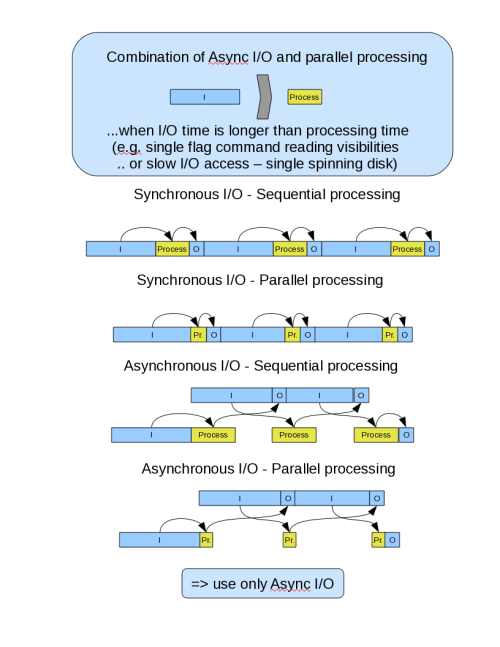
\includegraphics[scale=0.7]{async.parallel.diagram.IOdominates.png}
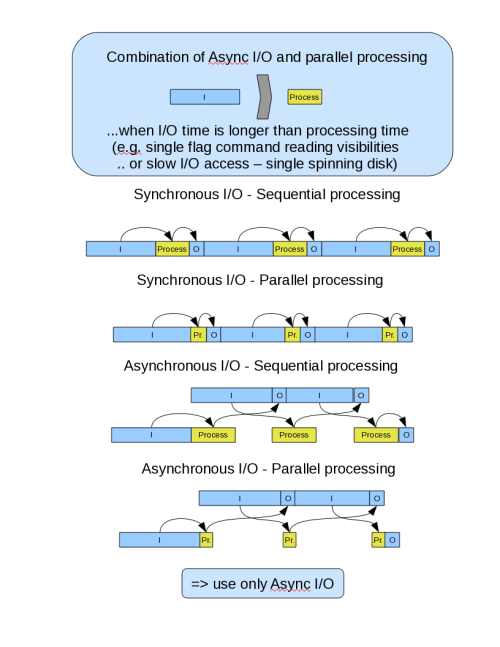
\includegraphics[scale=0.7]{async.parallel.diagram.IOdominates.png}
\caption{Explanation...}
\label{Fig:AsyncDiags}
\end{figure}






\subsubsection{Timing Tests}

Data : 

Continuum : few fat channels.\\
SpectralLine : many thin channels.\\

SinglePointing : contiguous scans on the same field\\
Mosaic  :  each scan is a different fields.\\

\begin{enumerate}
\item \label{dA} L-band continuum , Single Pointing   ----- need to decide dataset (probably G55.7+3.4\_1s.ms)
\item \label{dB} L-band spectral-line , Mosaic            ----- need to pick dataset 

\end{enumerate}


\paragraph{Comparison between modes}
{\green Tables from Justo for 50 and 150 GB continuum datasets. }


\begin{figure}
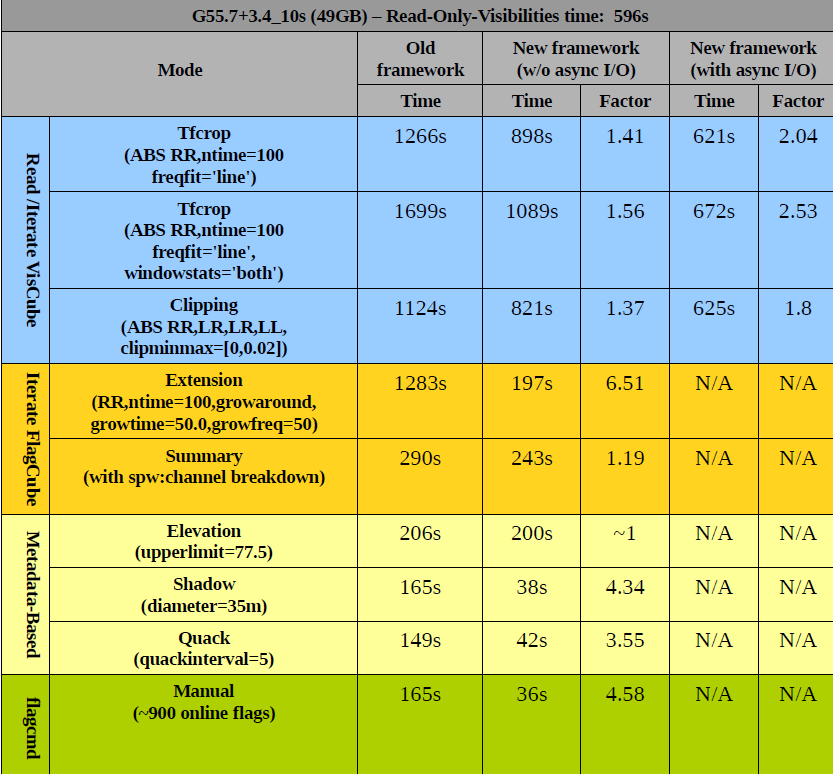
\includegraphics[scale=0.7]{table.timings.50GB.G55data.png}
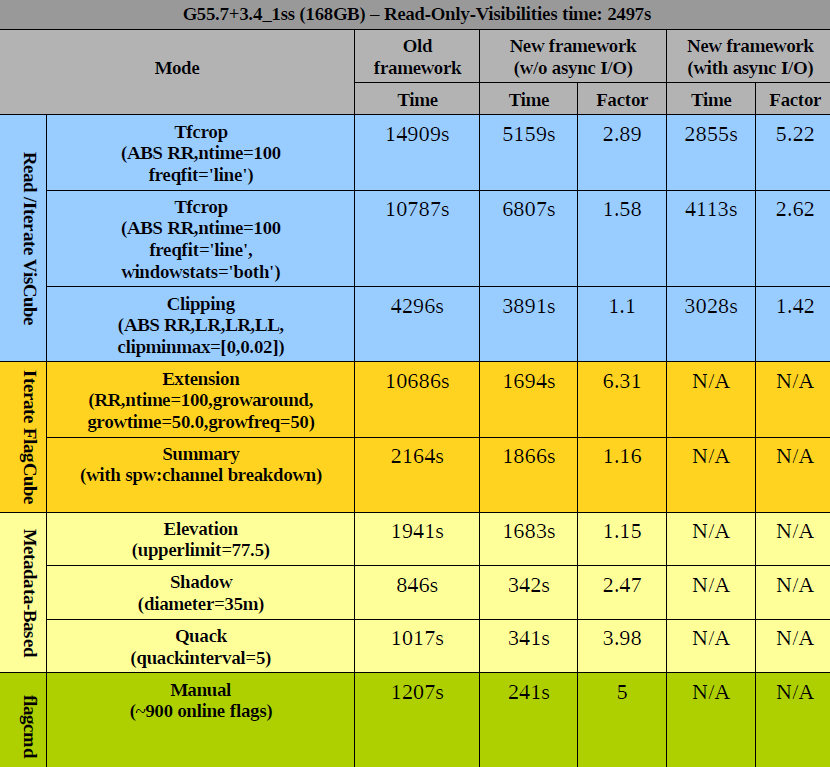
\includegraphics[scale=0.7]{table.timings.150GB.G55data.png}
\caption{These tables show timing comparisons between various modes, for two EVLA continuum datasets. Parameters of the datasets are... }
\end{figure}


\paragraph{Break-down of timings} : if possible, with and without async-IO.
\begin{enumerate}
\item  Only-reading-visibilities 
\item  Only-reading flags
\item  Only-writing flags
\item  (pls ignore if this makes no sense.) Only-iterating through the visbuffers without reading/writing anything (i.e. to see if much time is saved by the loose union). 
\end{enumerate}

\paragraph{Comparison between data-shapes and iteration patterns}

Two types of datasets : wideband continuum single-pointing,   spectral-line mosaic



%%%%%%%%%%%%%%%%%%%%%%%%%%%%%%%%%%%%%%%%%%%%%%%%%%%%
%%%%%%%%%%%%%%         SECTION           %%%%%%%%%%%%%%%%%%%%%%%%%%%
%%%%%%%%%%%%%%%%%%%%%%%%%%%%%%%%%%%%%%%%%%%%%%%%%%%%



\subsection{Python tool and task}

{\green Link to (or copy of) Sandra's documentation of the tool/task design and usage pattern }

\subsubsection{tflagger tool}

\begin{enumerate}
\item    Examples how to use the the new flagging framework from the tool.

\item    Explain what things can only be done from the tool level 

\item    Explain the heuristics applied for the automatic activation of async I/O and parallel run
\end{enumerate}

\subsubsection{flaghelper class}

\subsubsection{tflagdata task}

\subsubsection{tflagcmd task}



%%%%%%%%%%%%%%%%%%%%%%%%%%%%%%%%%%%%%%%%%%%%%%%%%%%%

